\section{ANITA detector model}
\label{sec:ANITA}
Taking into account the payload rotation, the simulated signal is
propagated to the front of each of the ANITA antennas and through the trigger and digitizer paths of the ANITA instrument.
The payload position chosen along the flight path is used to load appropriate information about the payload rotation, channel threshold values and channel masking.
The payload geometry is simulated using photogrammetry measurements
and phase-center calibration measurements taken with a ground pulser
during the flights.
Antenna gains measured in the lab previous to the flight are
applied to the signal according to the incident angles on the E and H planes. 

The signal then follows the signal chain as shown in
Figure~\ref{fig:ANITA3_signalChain}.
First, the incident fields are folded into the vertical-polarization (VPOL) and horizontal polarization (HPOL) responses of the antennas. 
The responses of these paths are divided into the trigger and digitizer
paths.
The digitizer and trigger responses were measured using calibration data taken before
the flights. 
Figure~\ref{fig:ANITA_ImpulseResponses}~(left) shows the
power spectra of the trigger and digitizer impulse responses for a
sample channel of the ANITA-III payload.
To avoid continuous wave (CW) noise from satellite and station transmissions, ANITA-IV adopted 
tunable notch filters (see Section~\ref{subsec:tuffs} and Reference~\cite{Allison:2017vtk}).
Figure~\ref{fig:ANITA_ImpulseResponses}(right) shows the
power spectra of the trigger and digitizer impulse responses for a
sample channel of the ANITA-IV payload with the most common filter configuration used during flight.
Thermal noise is generated based on flight measurements (see Section~\ref{subsec:ANITA_thermalNoise}) and added to the waveforms.
The modeled tunnel diode response (see Section~\ref{subsec:ANITA_trigger}) is convolved with the signal waveforms from all the channels, and if an event passes the trigger logic, the event is saved in the final output.

\begin{figure}[!h]\centering
  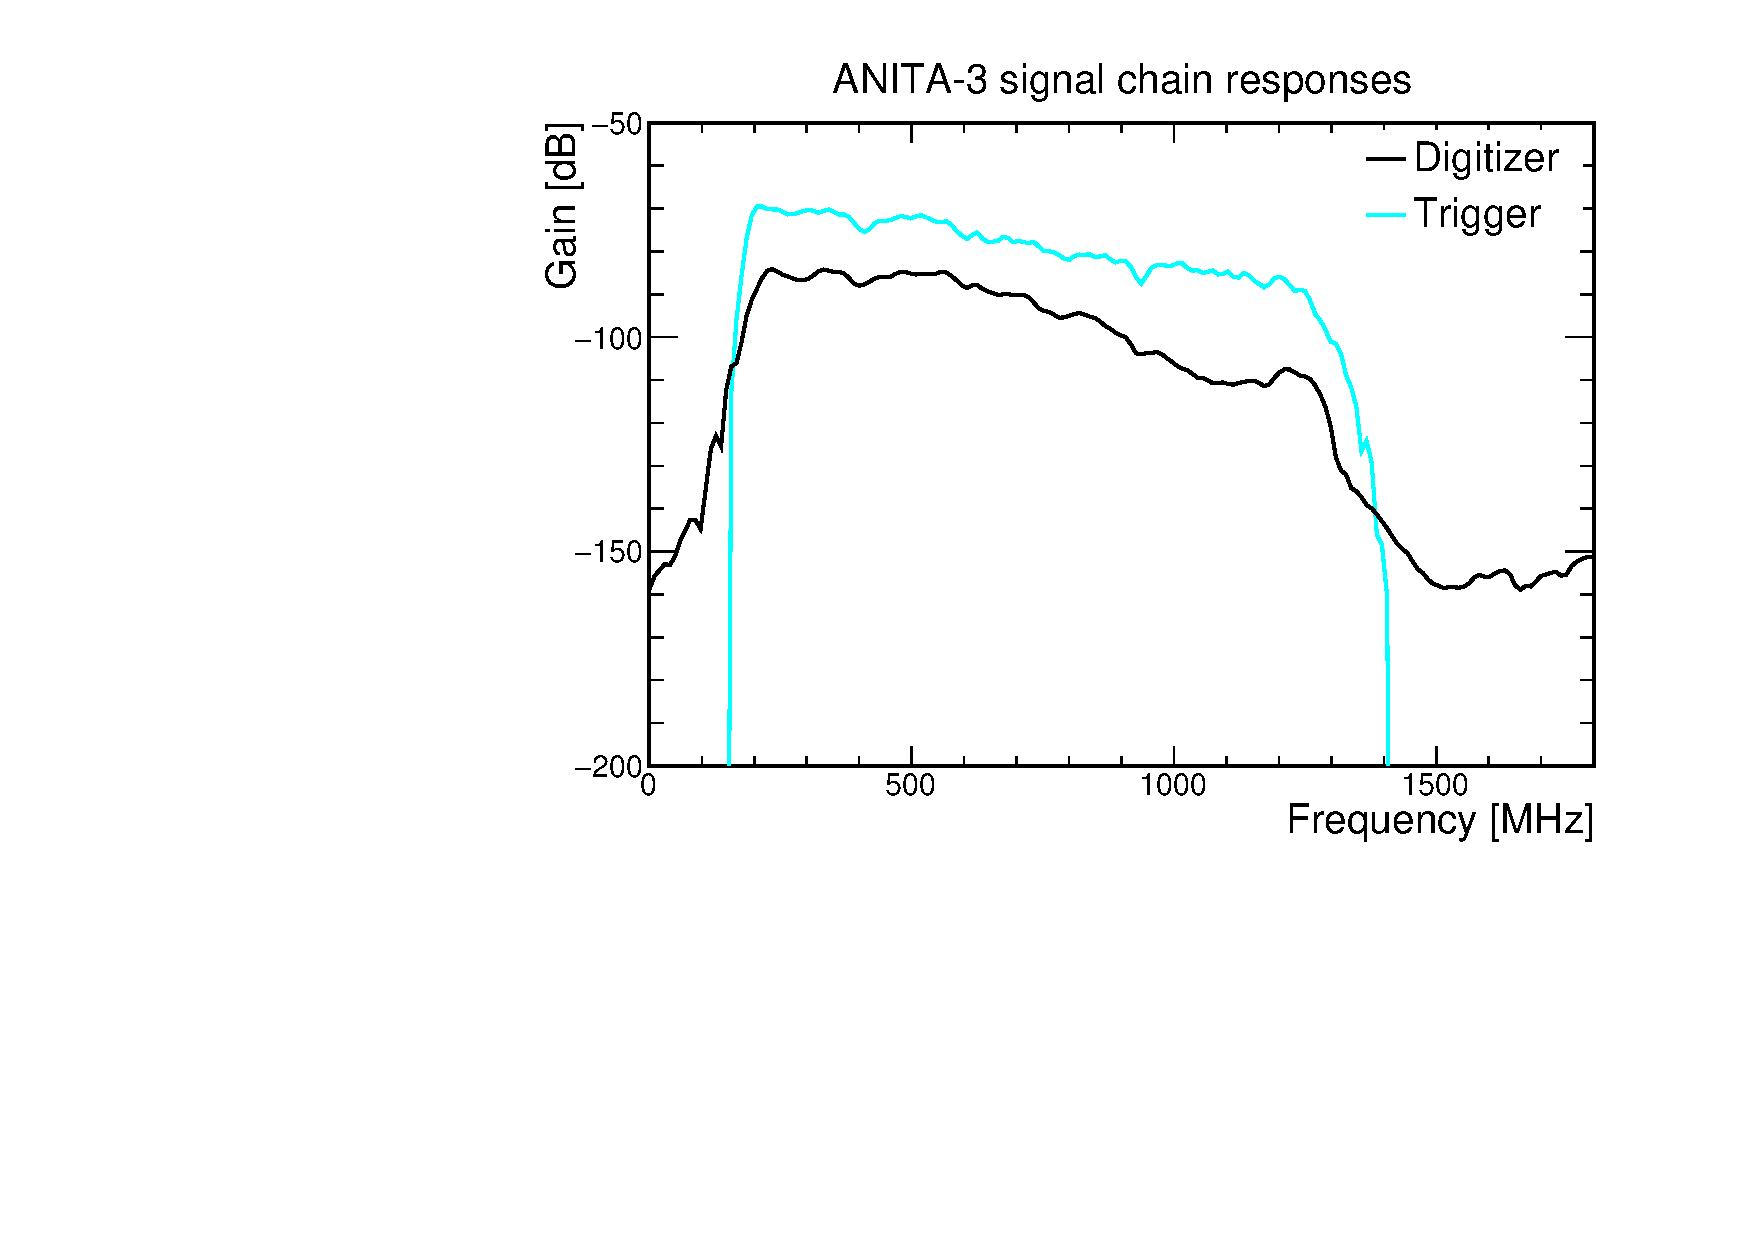
\includegraphics[width=.45\linewidth]{./Figs/A3ImpulseResponses.pdf}
  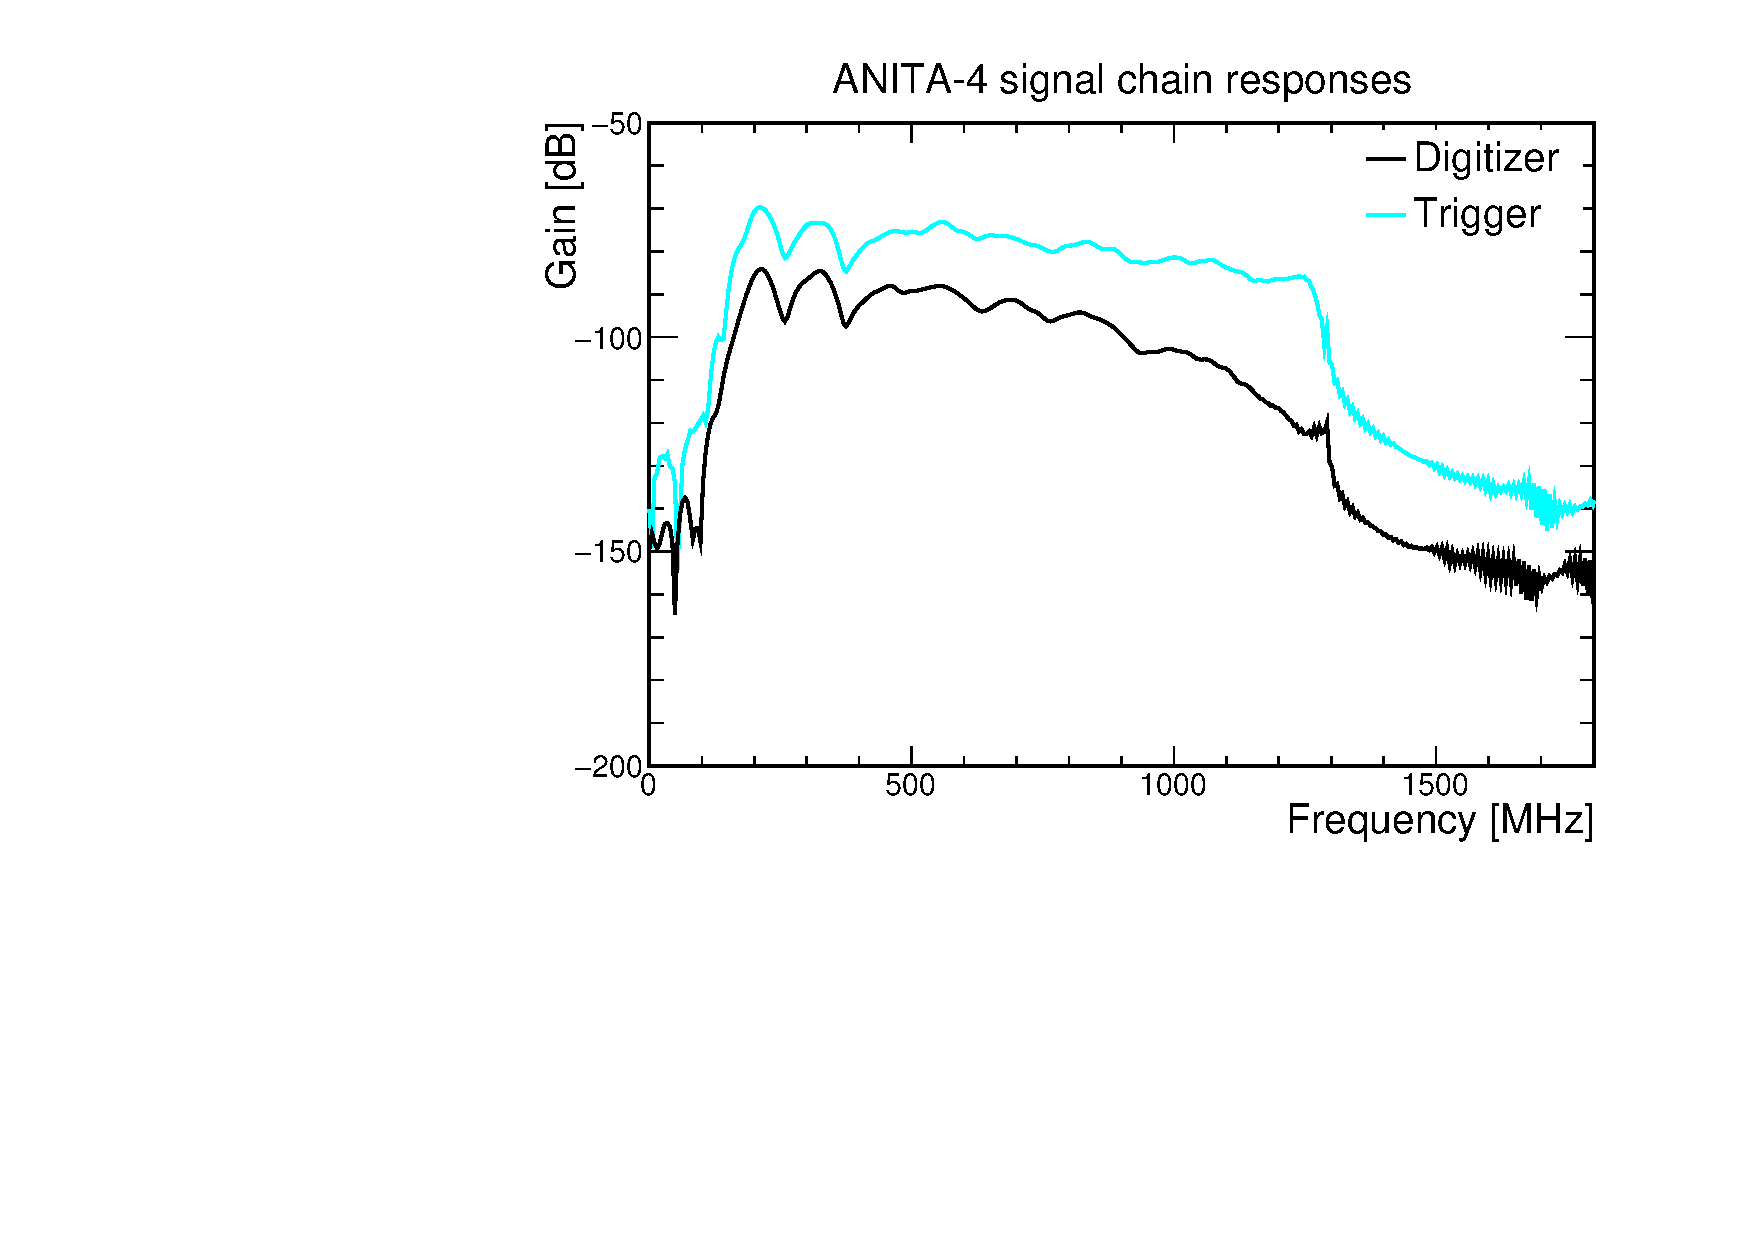
\includegraphics[width=.45\linewidth]{./Figs/A4ImpulseResponses.pdf}
  \caption{Power spectrum of the trigger and digitizer impulse
    response for a sample channel, for the ANITA-III (left) and ANITA-IV (right) instruments. 
    %\CD{Why is there power above Nyquist?}
    }
  \label{fig:ANITA_ImpulseResponses}
\end{figure}


\subsection{Tunable Universal Filter Front-end boards}
\label{subsec:tuffs}
To alleviate the anthropogenic noise observed in ANITA-III that caused
significant amounts of deadtime, ANITA-IV added the Tunable Universal
Filter Front-end, or TUFF, boards~\cite{Allison:2017vtk}.
This board uses up to three notches to attenuate
the gain by a maximum of 13\,dB around each notch
frequency:
the notches are tunable, but default to 260, 375, and 460\,MHz  (corresponding to known satellite communications frequencies) using LRC circuits. 
Whether each notch is activated and at which frequency (they
can be moved to non-default positions) is called
a "configuration".
There were seven unique configurations for the ANITA-IV flight  which are simulated in 
\icemc. 
The response of the trigger for the configuration when all notches are on and at default frequencies is plotted in Figure~\ref{fig:TUFFs}(left). 
An example of the effect of the third notch switched on or off when 460\,MHz carrier wave noise is simulated is shown in Figure~\ref{fig:TUFFs}(right).

The time-dependent response for each channel for a given configuration is loaded into \icemc and convolved with the trigger and digitizer impulse responses. 

\begin{figure}
  \centering
 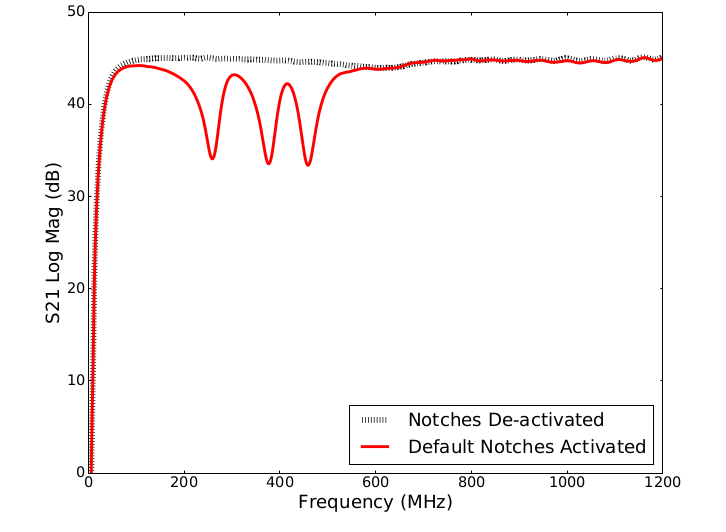
\includegraphics[width=0.45\linewidth] {./Figs/config_P_response_freq.png} 
 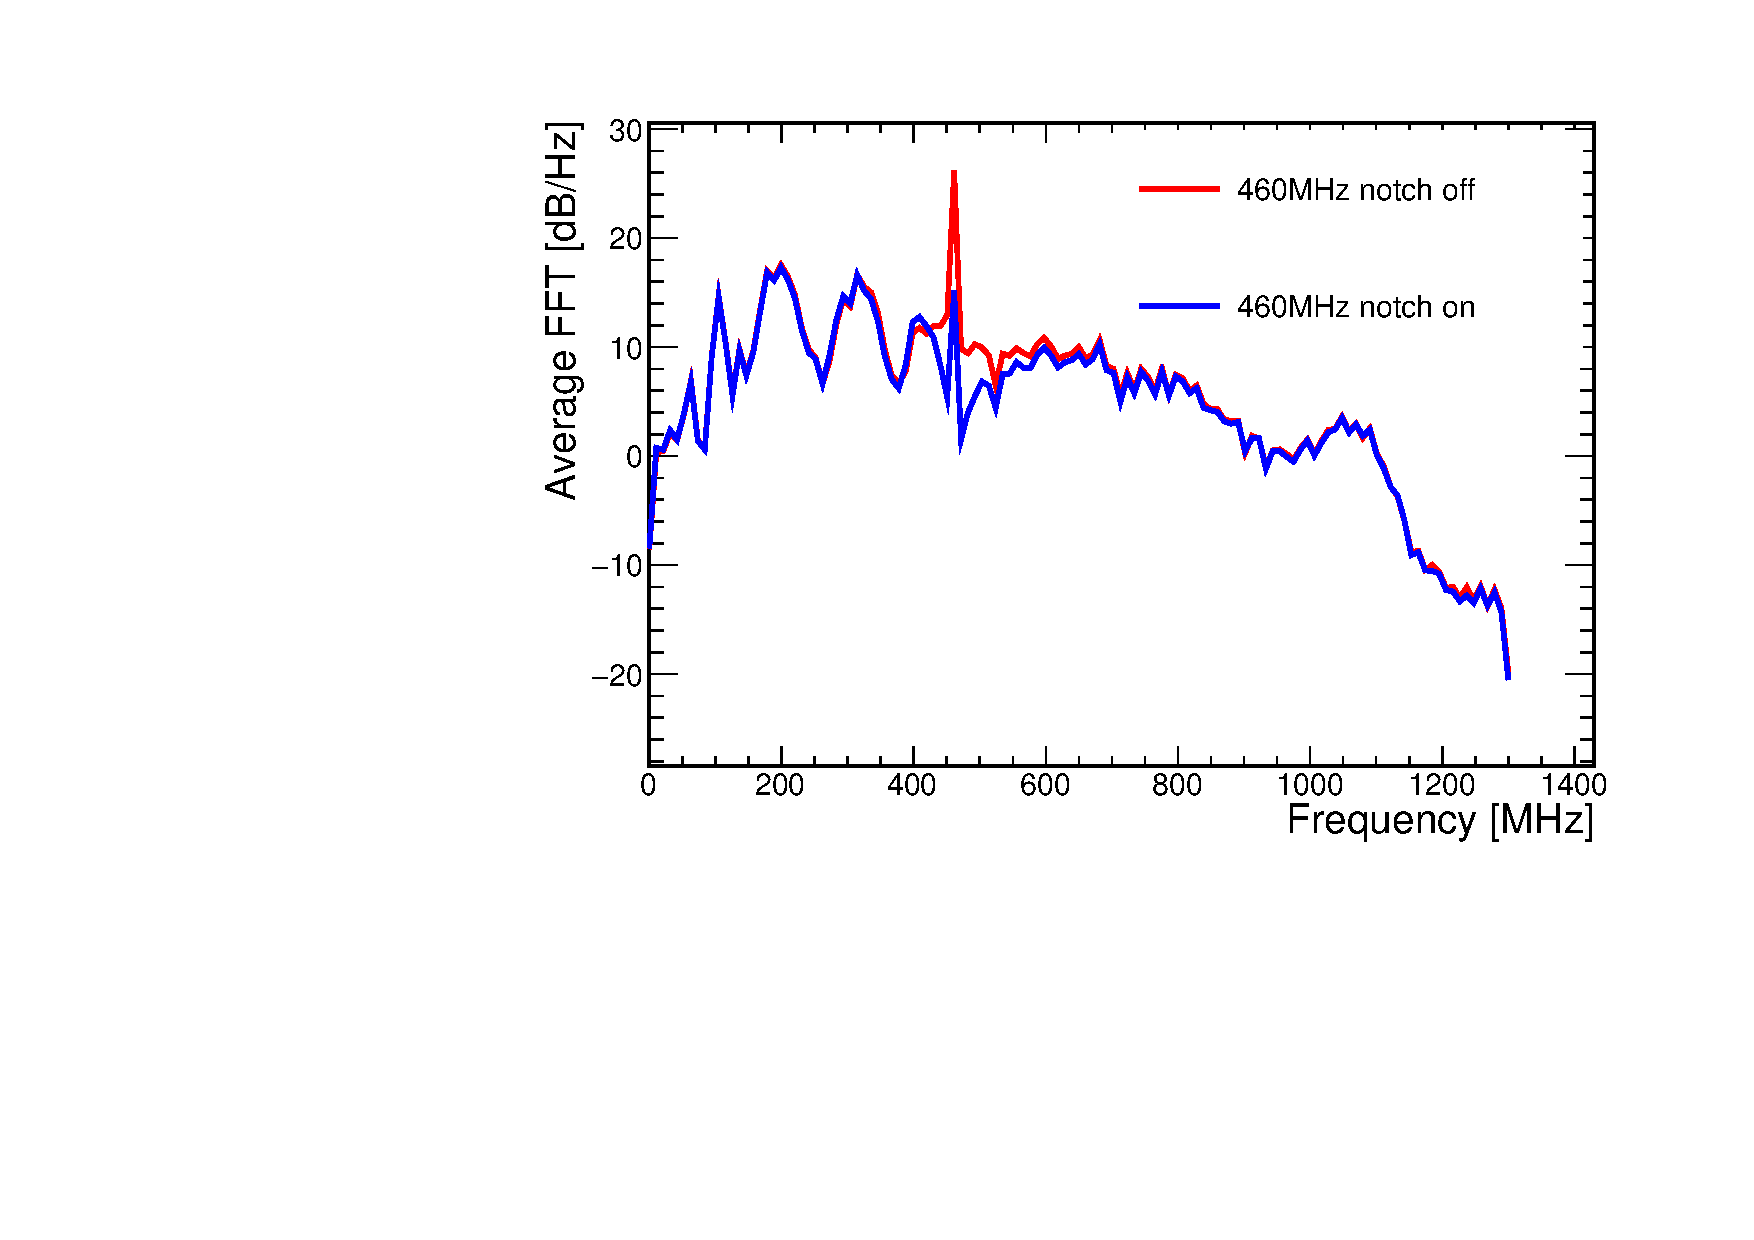
\includegraphics[width=0.45\linewidth] {./Figs/Icemc_tuffs.pdf} 
  \caption{(Left) TUFF response in frequency domain (dB vs frequency). The dips in the response clearly mark the 260, 375, and 460 MHz notches turned on in this configuration~\cite{Allison:2017vtk}.
  (Right) Example of carrier wave noise injected in \icemc with the third notch activated or not activated.}
\label{fig:TUFFs}
\end{figure}



\subsection{Thermal noise}
\label{subsec:ANITA_thermalNoise}
Modelling thermal noise is crucial to the simulation of
neutrinos as it affects both the trigger and analysis efficiencies.
An accurate model of the thermal noise makes it possible to simulate both the
accidental noise triggers and the effect of noise fluctuations on the
reconstructed correlation maps used to calculate the event direction in the ANITA analyses~\cite{romero2015interferometric}.

To accurately model the thermal noise during the ANITA flights, events coming from minimum bias triggers during
a quiet time of the ANITA-III flight (runs 204-250, approximately 2.5
days) are used to produce power spectra for each digitizer channel
using bins of width 10\,MHz.
As the ANITA-III flight suffered more than the previous flights 
from continuous wave noise coming
from satellites and human bases, frequencies in the ranges
234-286\,MHz and 344-410\,MHz are filtered out in software analysis
using two simple notch filters. 
Antennas facing the sun were also excluded from the average.

For each channel and each frequency bin a Rayleigh PDF is fit to the data:
\begin{equation} 
  f(A, \sigma)=\dfrac{A}{\sigma^2}e^{-A^2/(2\sigma^2)} \;,
  \label{eq:rayleigh}
\end{equation}
\noindent where $A$ is the amplitude in the frequency domain (in mV/MHz) and $\sigma$ is the
Rayleigh amplitude in that frequency bin.
As most of the carrier wave noise is in the tail of these
distributions, the Rayleigh fits are performed only to the rising edge and peak of the distributions.
Figure~\ref{fig:rayleighFits}(left) shows an example of Rayleigh distribution fits for a sample channel in the frequency bin centred at 710.94\,MHz.
Events in this sample come from minimum bias triggers during the ANITA-III quiet time.
 
\begin{figure}[!h]\centering
  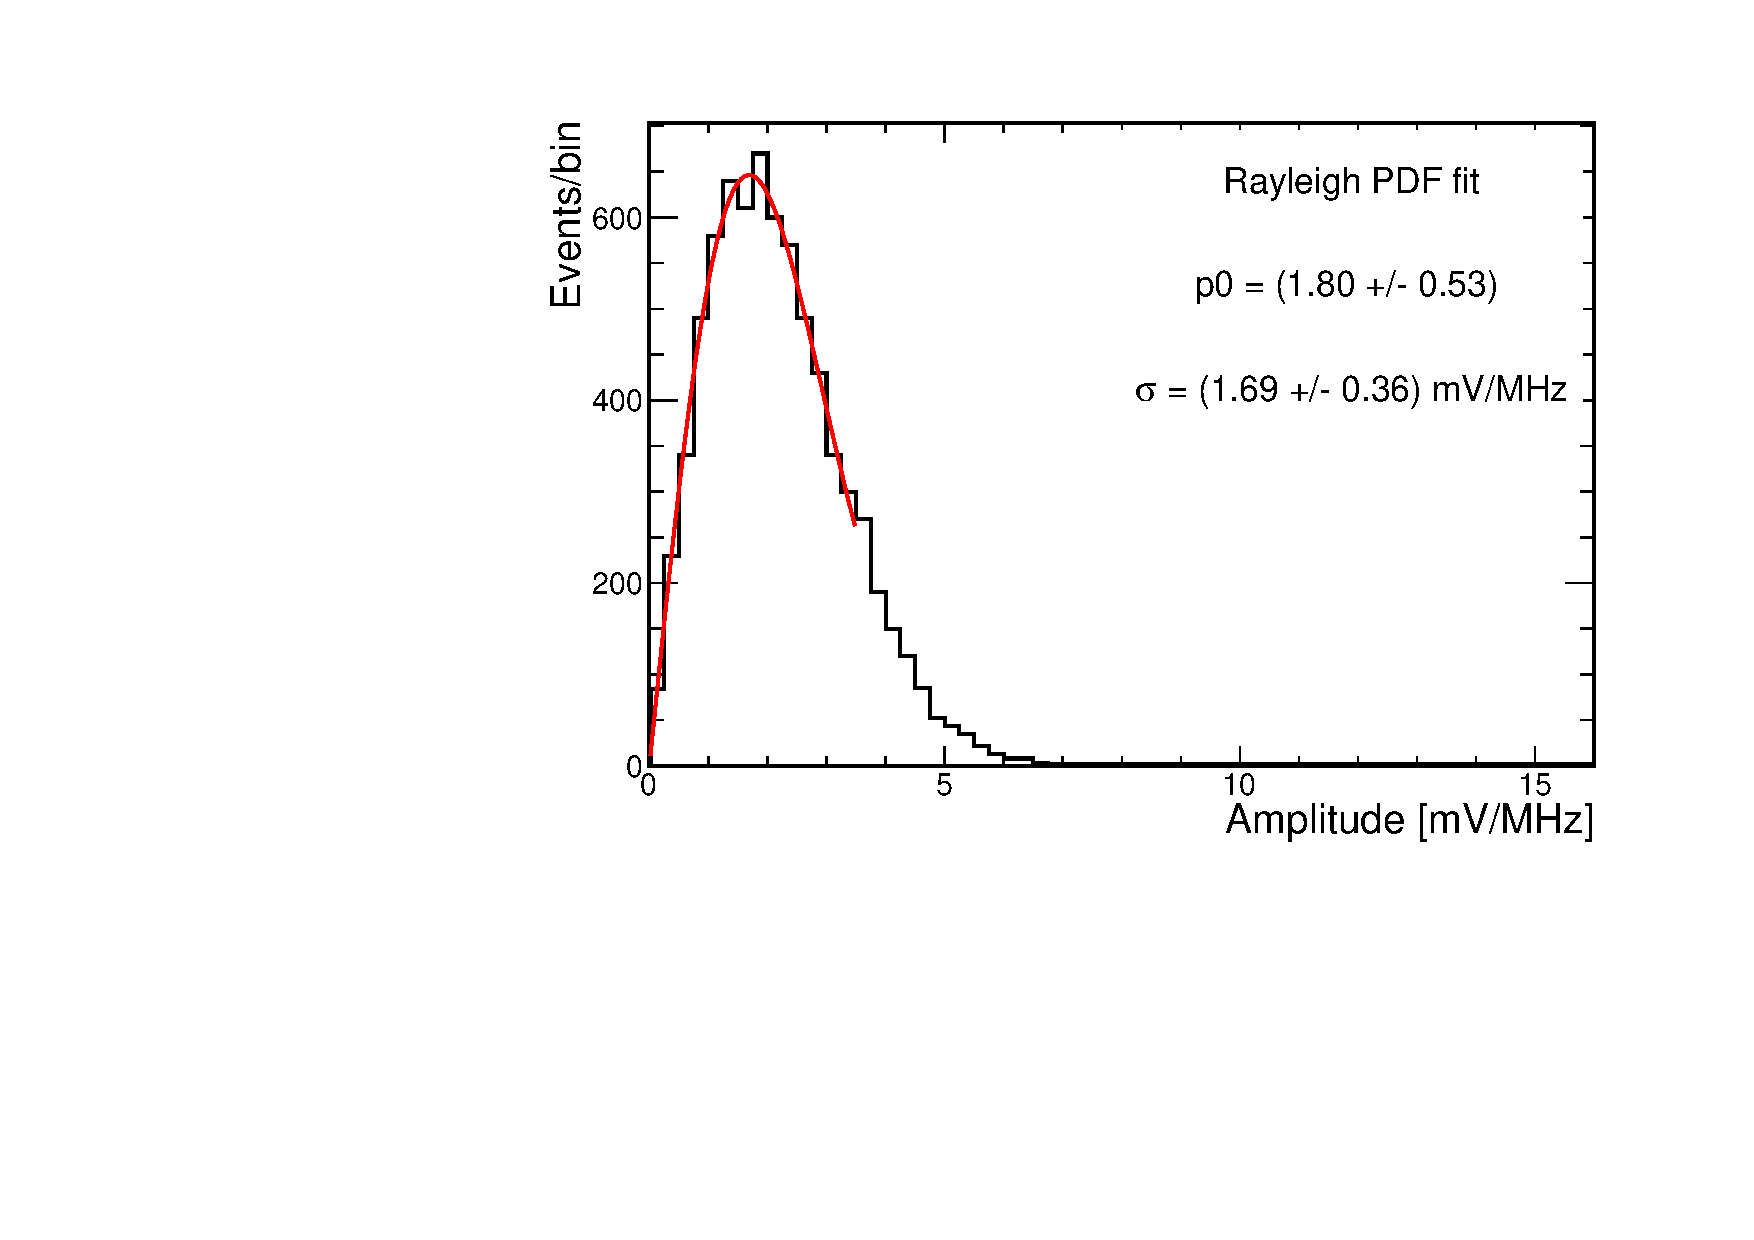
\includegraphics[width=.45\linewidth]{./Figs/RayleighExample.pdf}
  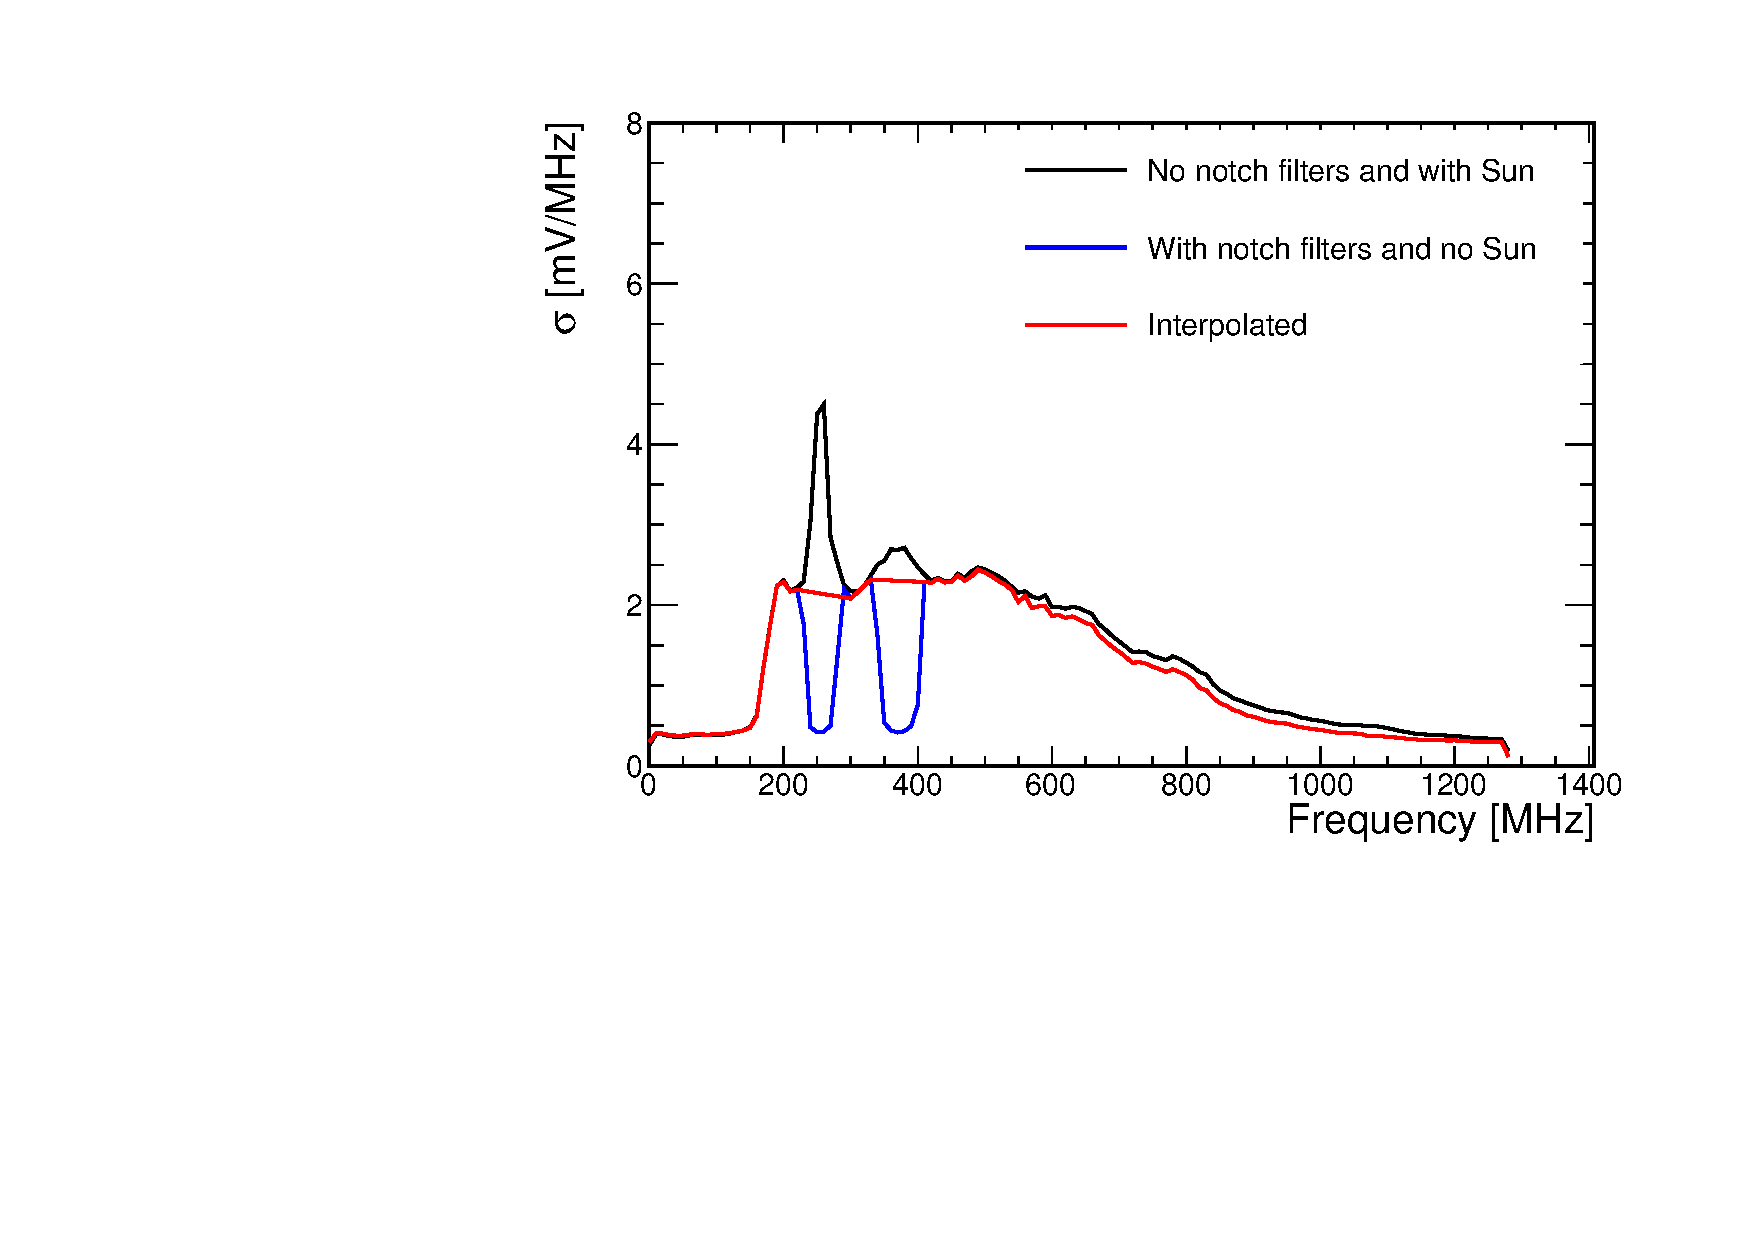
\includegraphics[width=.45\linewidth]{./Figs/RayleighSigma_1V_old.pdf}
  \caption{Example of a Rayleigh fit for a sample channel in the
    710.94\,MHz frequency bin (left). The fit is performed only to the rising edge and peak of the distributions, as most CW noise in in the tail. 
Right: fitted amplitude, $\sigma(f_i)$, as a
    function of frequency (interpolating in the frequency range where power is filtered). }
  \label{fig:rayleighFits}
\end{figure}

Graphs of the fitted amplitude, $\sigma(f_i)$, as a function of
frequency were produced for each channel (interpolating in the frequency range where power is filtered), as seen in Figure~\ref{fig:rayleighFits}(right).
In \icemc these graphs are used to generate random noise in the
frequency domain for each channel: for each frequency bin $f_i$ the real and imaginary part are randomly extracted from a Gaussian distribution with zero mean and amplitude
%\begin{equation} 
%  \begin{split}
%    \Re{f_i} & = RandomGaus(0, \sigma(f_i))/\sqrt{N_f} \\
%    \Im{f_i} & = RandomGaus(0, \sigma(f_i))/\sqrt{N_f} \\
%  \end{split}
%  \label{eq:thermalNoise}
%\end{equation}
%\noindent where $f_i$ is a frequency bin,
$\sigma(f_i)$, the fitted Rayleigh amplitude in that bin.
%and $N_f$ is the total number of frequencies.

This noise is added to the signal in the digitizer path.
For the trigger path the noise is re-normalised using the bin-by-bin ratio of the
trigger to digitizer path impulse response in the frequency domain
before adding it to the signal.

Thermal noise for the ANITA-IV simulation is derived from the ANITA-III measurements, accounting for the different electronics response (including the use of low noise amplifiers and variable filter configurations during the flight) for the two missions.
Samples containing only thermal noise are also produced, and they are used in
the main ANITA analyses to test the robustness of our analysis selection.
Subsection~\ref{subsec:validation_flight} details the thermal noise validation for both ANITA flights.

%While producing Rayleigh fits to all channels, it turned out that two
%channels (T04V and T04H) showed a different behavior than all the
%others, as shown in Figure~\ref{fig:noiseWeird}.
%T04V showed very irregular behavior during the whole flight (coming
%off and on at different periods), while T04H is the channel with the
%ALFA antenna attached to it, hence all frequencies above 700\,MHz were
%filtered out.
%For the moment these two graphs are used to simulate thermal noise in these two
%channels for the ANITA-III flight. 
%\begin{figure}[!h]\centering
%  \includegraphics[width=.45\linewidth]{/Users/linda/ANITA/anita3/anitaBuildTool/RandomMacros/powerSpectra/plots/RayleighSigma_4V.png}\,
%  \includegraphics[width=.45\linewidth]{/Users/linda/ANITA/anita3/anitaBuildTool/RandomMacros/powerSpectra/plots/RayleighSigma_4H.png}
%  \caption{Graphs of the fitted amplitude ($\sigma(f_i)$) as a
%    function of frequency for channels T04V and T04H (interpolating
%    between filtered frequencies).}
%  \label{fig:noiseWeird}
%\end{figure}

%\subsection{Anthropogenic noise} 
%\label{subsec:ANITA_anthropogenicNoise}



\subsection{Trigger simulation}
\label{subsec:ANITA_trigger}
The simulation models the L0 trigger by passing the
trigger-path signal through a time-domain tunnel diode model and comparing it to the
appropriate threshold from the flight for that channel at the event
time.
The tunnel diode response can be thought of as an integral of the power over about 10\,ns, but the true response is non-trivial.
The tunnel diode response function is constructed based on the trigger diode output for each channel.
The shape of the diode response is described by the sum of two negative Gaussians and a positive function that is the product of a quadratic and an exponential:
\begin{equation}
      f(t) = A_1 \cdot e^{-(t-t_0^1)^2/2\sigma_1^2} + 
      A_2 \cdot e^{-(t-t_0^2)^2/2\sigma_2^2} +
      A_3 \cdot \left( t-t_0^3 \right)^2 \cdot
      e^{-(t-t_0^3)/\sigma_3} \;,
    \end{equation}
\noindent where the values for the parameters are shown in
Table~\ref{tab:diodeModelParameters};
$f(t)$ is dimensionless.
Reference~\cite{diodeModel} describes how the model was found. Figure~\ref{fig:ANITA_diodeModel} shows the diode response model function.

\begin{table}[h!]
\caption{Tunnel diode model parameters used for the full band trigger in ANITA-III and ANITA-IV.}
  \begin{center}
    \begin{tabular}{c|c|c|c} 
      & Value 1 & Value 2 & Value 3 \\
     \hline
      $A$           & -0.8  & -0.2   &  0.00964   \\
      $\sigma$ [ns] &  2.3  &  4.0   &  7.0       \\ 
      $t_0$  [ns]   & 15.0  & 15.0   & 18.0       \\
    \end{tabular}
  \end{center}
  \label{tab:diodeModelParameters}
\end{table}


\begin{figure}[!h]\centering
  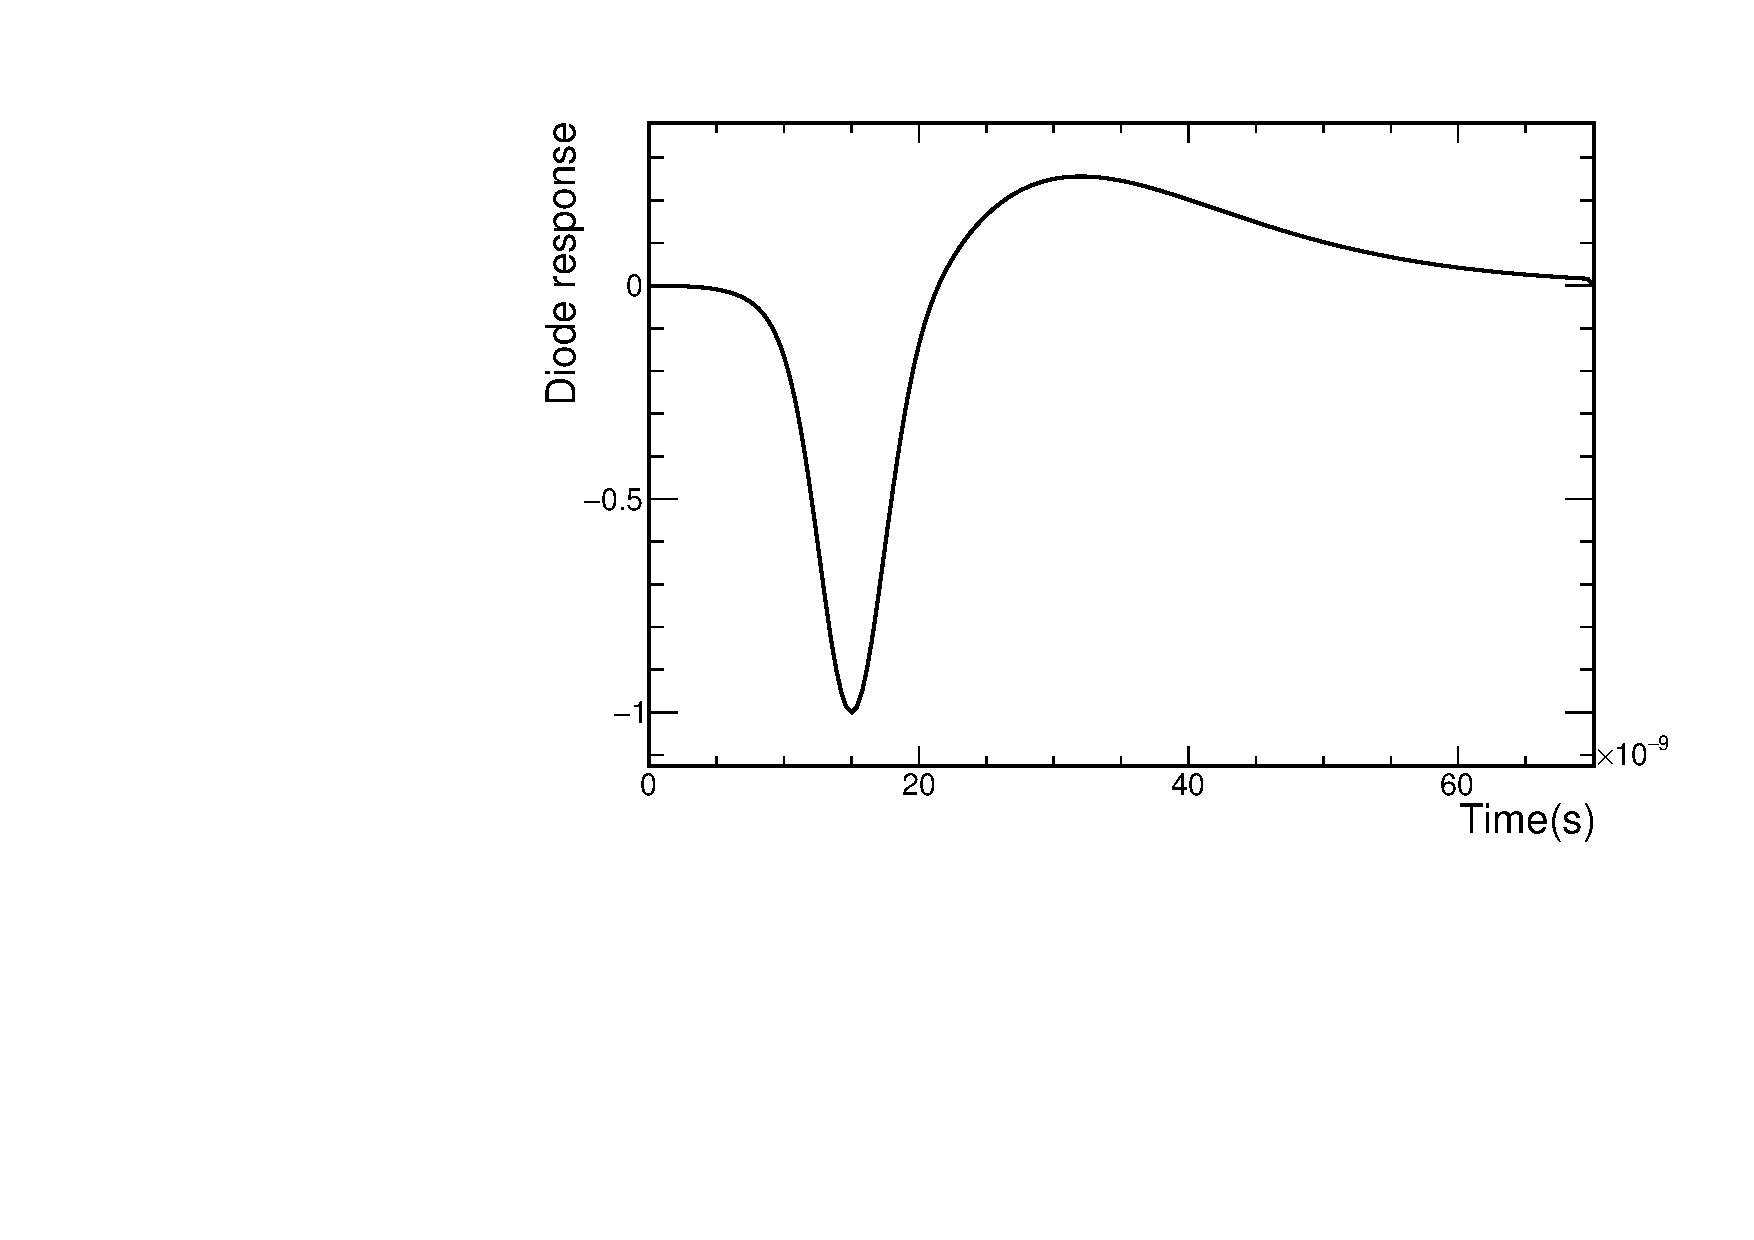
\includegraphics[width=.45\linewidth]{./Figs/FullBand_diodeResponse.pdf}
  \caption{Tunnel diode response model used in \icemc.}
  \label{fig:ANITA_diodeModel}
\end{figure}

For each waveform, the power as a function of time is calculated as:
\begin{equation}
  P (t) = \dfrac{V(t) \cdot V(t)}{Z} \;,
\end{equation}
\noindent where $V(t)$ is the voltage at time $t$, and $Z=50\,\Omega$ is the system impedance.
The next step is to convolve the waveform power with the diode
response to find the diode output $D(t)$:
\begin{equation}
  D(t) = (f * P)(t) \;.
\end{equation}
For each time bin, the diode output is compared to the channel
threshold, $V_T$, multiplied by RMS voltage of the diode outputs coming from pure thermal noise, $V_{RMS}$, following:
\begin{equation} 
  D(t) < V_T \cdot V_{RMS} \;.
\end{equation}
If the power output is lower than the threshold multiplied by the diode RMS at any point, then that channel passes the L0 trigger.
  See Figure~\ref{fig:ANITA_diodeOutput} for an example of diode
  output that does not pass the L0 trigger (left) and that does pass
  the L0 trigger (right).

\begin{figure}[!h]\centering
  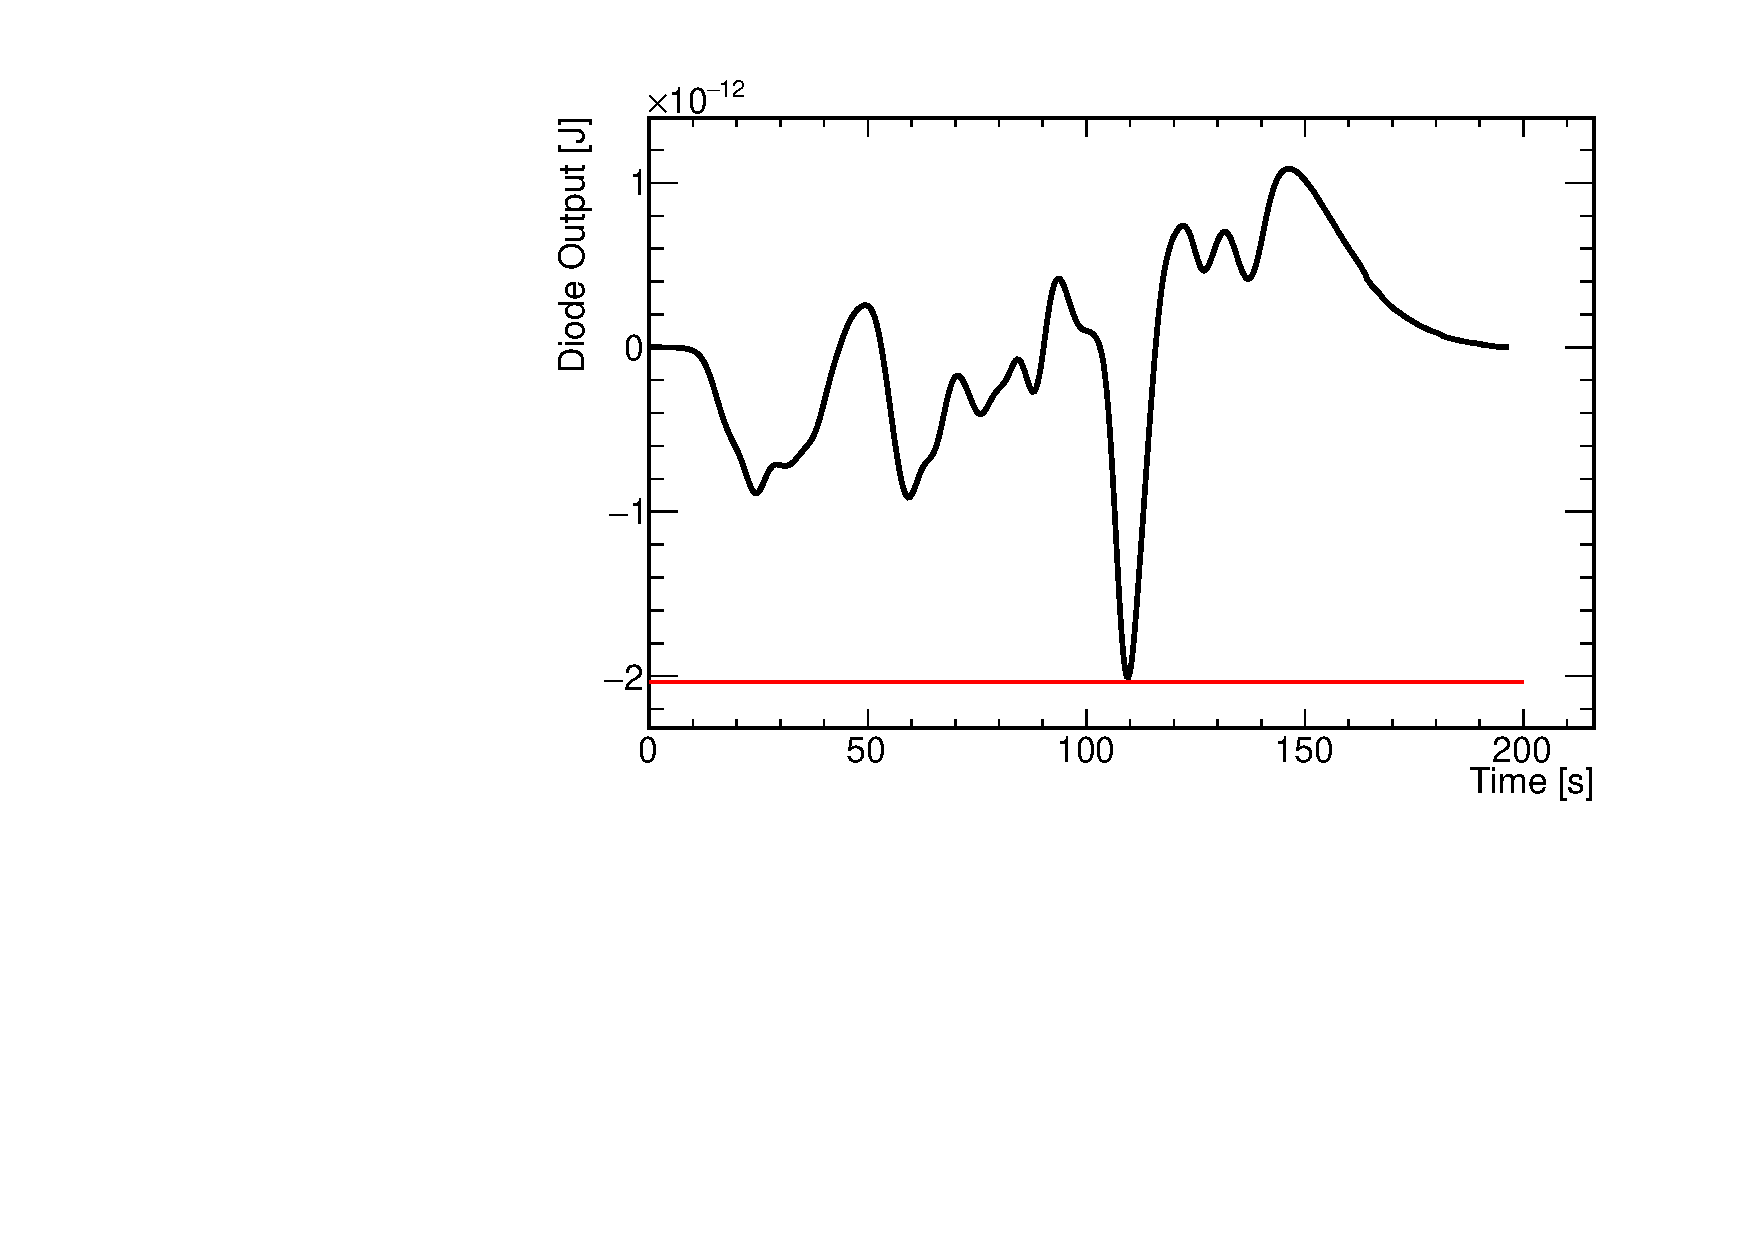
\includegraphics[width=.45\linewidth]{./Figs/ExampleDiodeOutput_NOpass.pdf}
  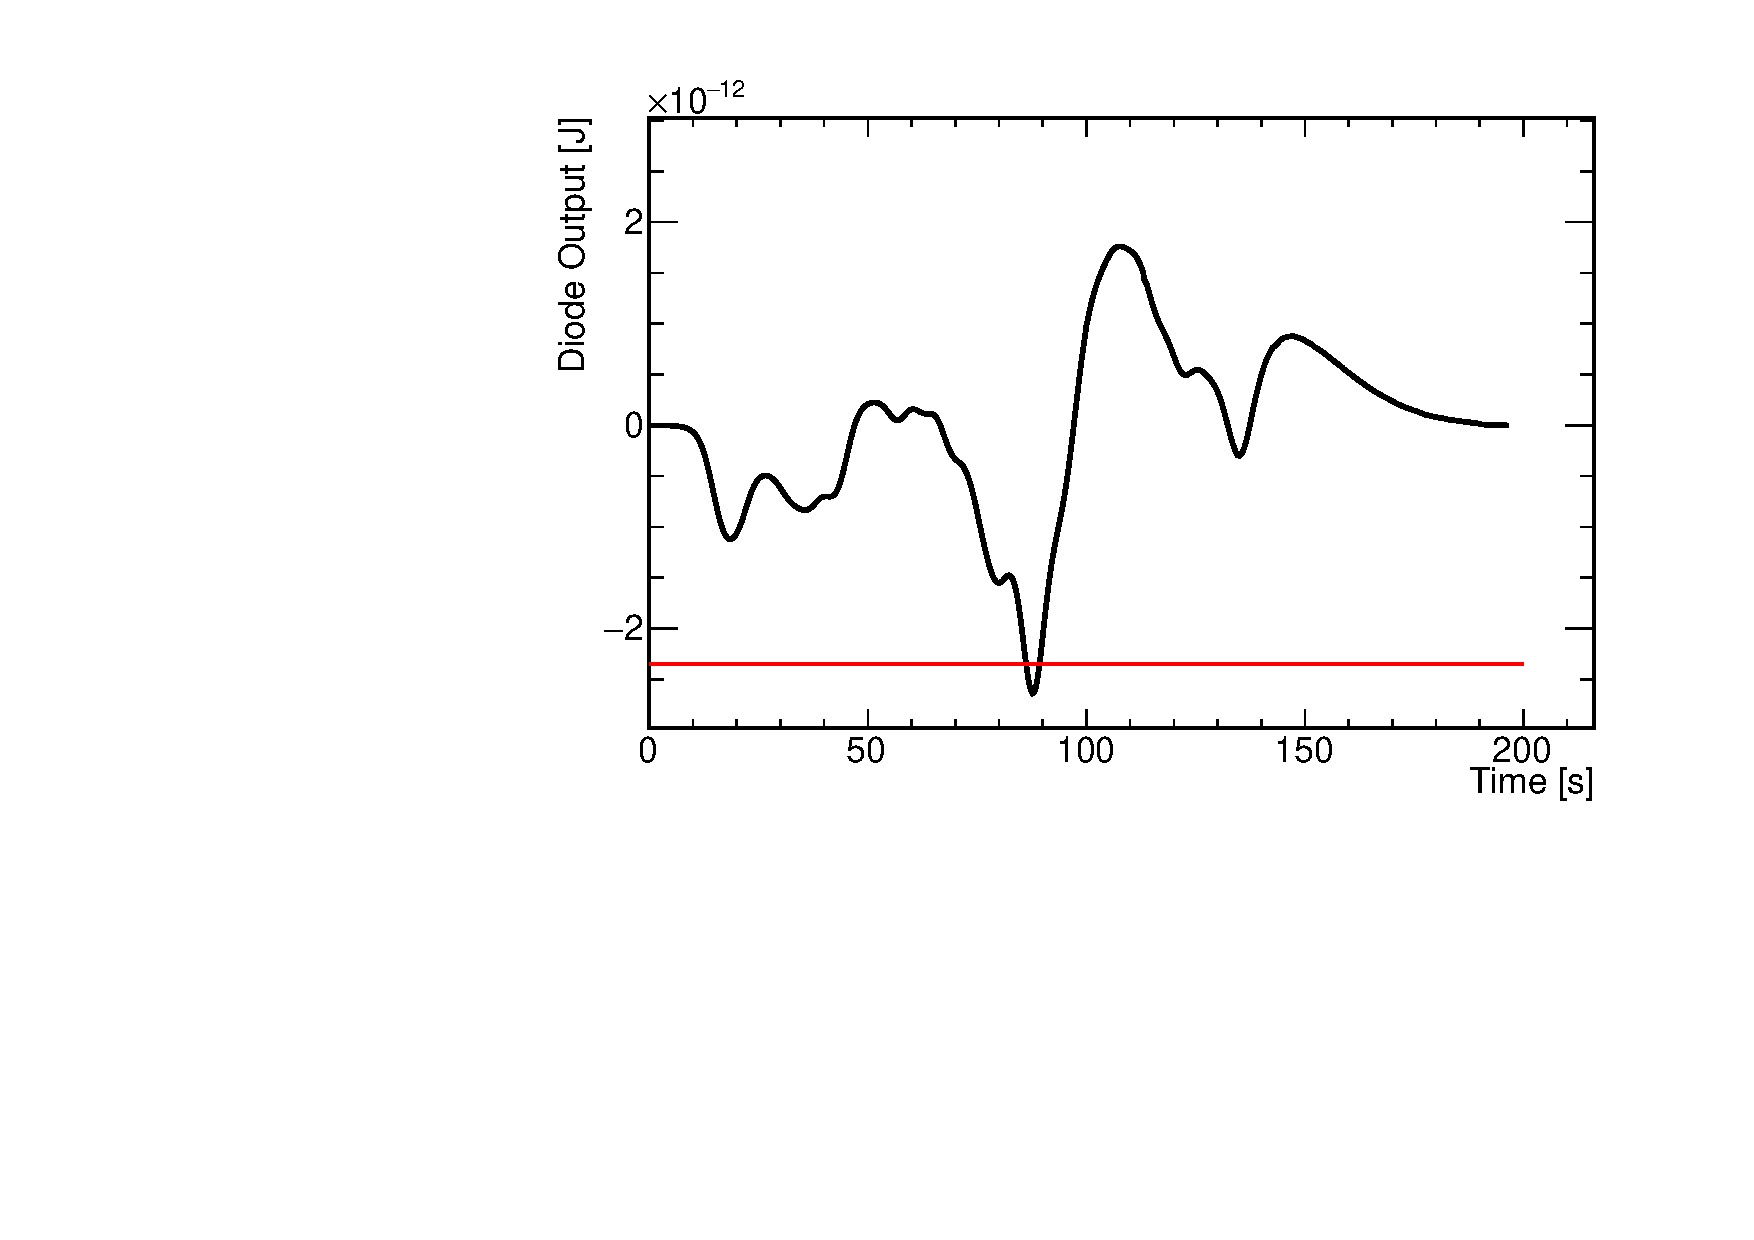
\includegraphics[width=.45\linewidth]{./Figs/ExampleDiodeOutput_pass.pdf}
  \caption{Example of typical diode output coming from a pure thermal
    noise waveform (left) and from a pulse (right). The red
    line shows the value of $V_T \cdot V_{RMS}$, showing that the
    waveform on the right passes the L0 trigger and the waveform on
    the left does not.}
  \label{fig:ANITA_diodeOutput}
\end{figure}

At the beginning of a run, $V_{RMS}$ is calculated for each channel 
by simulating 1000 noise waveforms
(Subsection~\ref{subsec:ANITA_thermalNoise}) 
and sampling the diode output at the center of each waveform
(see Figure~\ref{fig:ANITA_diodeRMS}).
In ANITA-III, two channels had very large $V_{RMS}$ associated with them that prevents them from triggering in the simulation: one was broken during the flight, and the other one had an additional filter applied during flight to
allow an in-flight calibration pulser to be used.

\begin{figure}[!h]\centering
  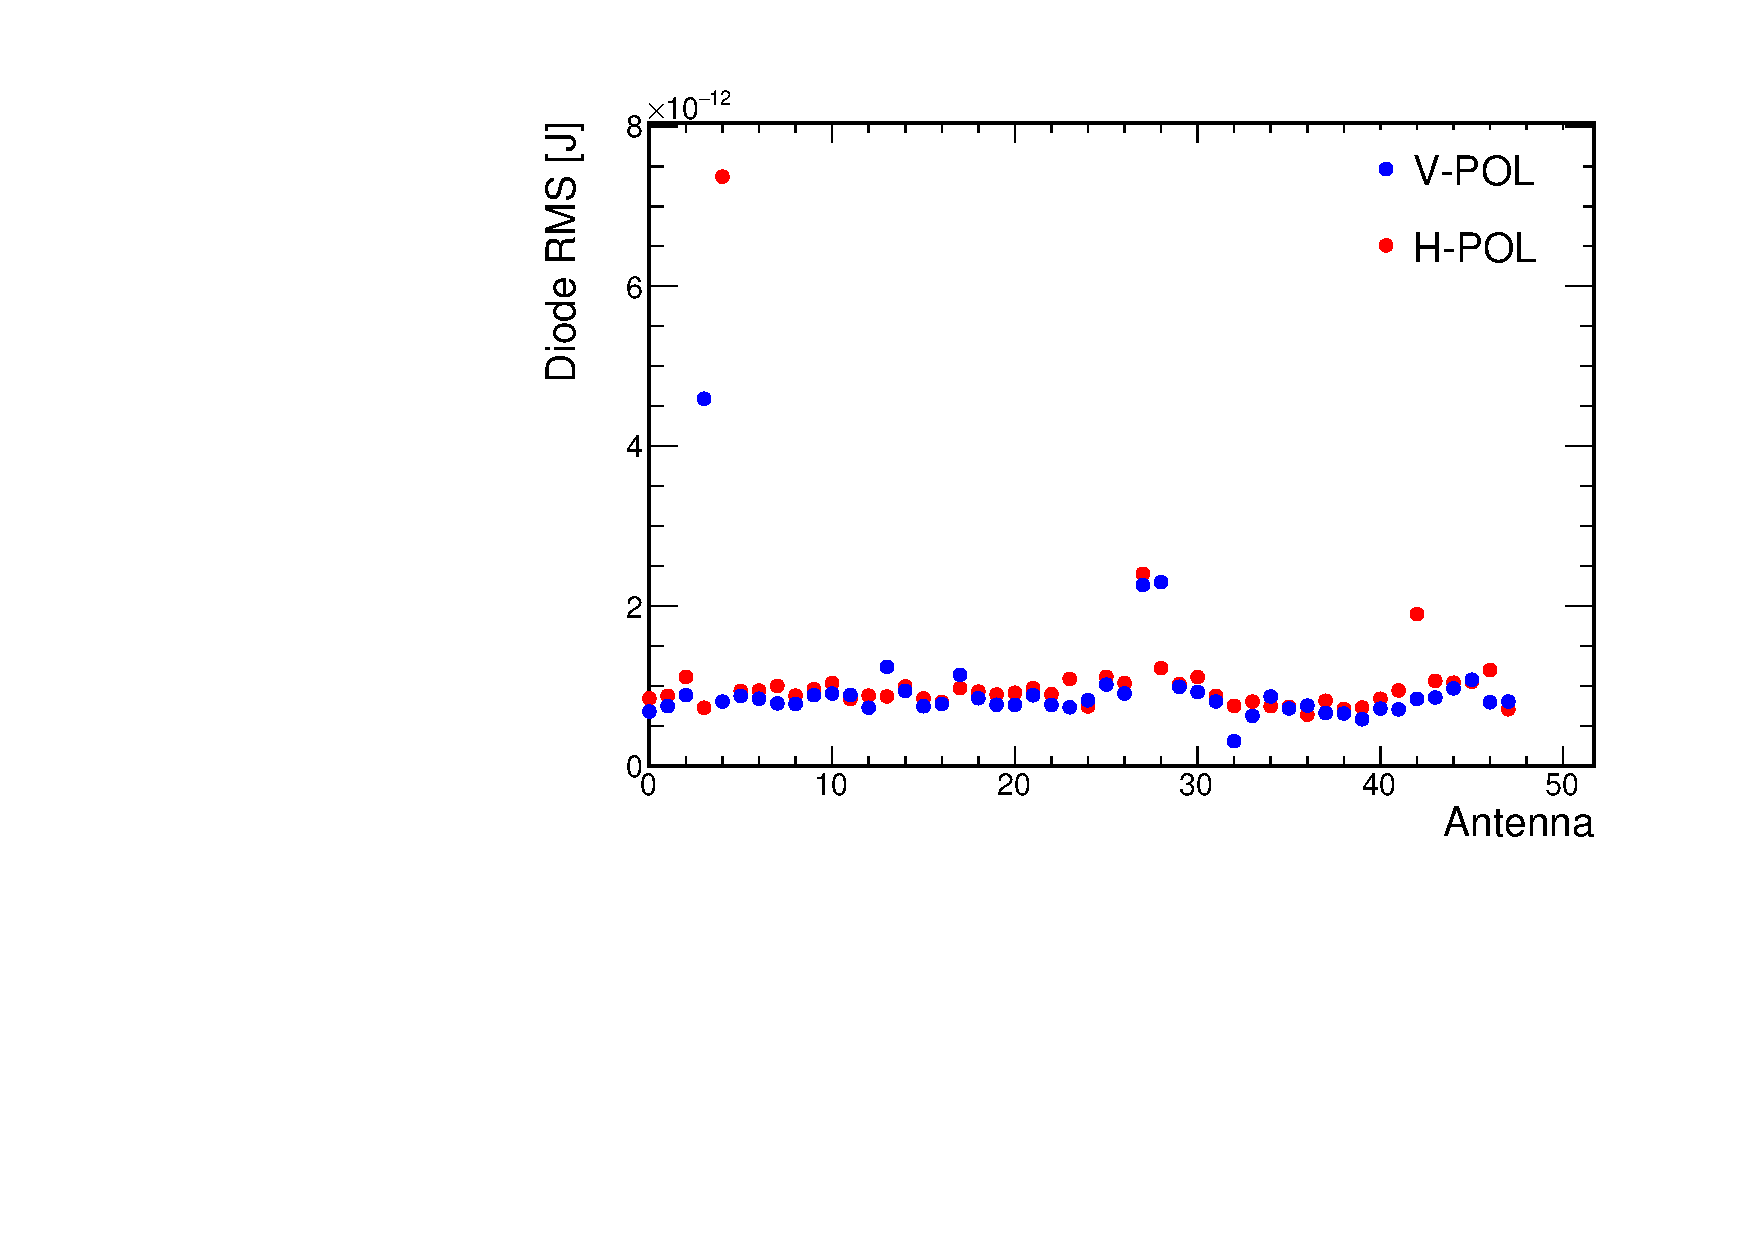
\includegraphics[width=.45\linewidth]{./Figs/DiodeRMSfromFile.pdf}
  \caption{Tunnel diode RMS for each channel. Channel 4 VPOL was broken during the ANITA flight; channel 5 HPOL had an additional filter applied to accommodate the use of an in-flight calibration system.}
  \label{fig:ANITA_diodeRMS}
\end{figure}
 
The trigger logic for the ANITA-III and ANITA-IV triggers is very similar.
The main difference is that ANITA-IV used 90 degree hybrids to transform HPOL and VPOL signals into LCP and RCP components of waveforms, so the ANITA-IV L1 trigger requires a LCP and RCP L0 coincidence in the same antenna within one 4\,ns clock cycle.
The ANITA-III instrument did not have an L1 trigger.
The L2 trigger is formed by a coincidence of two out of three
antennas (top, middle, bottom) in the same azimuthal
sector. As ANITA is intended to look for plane-waves from below, a simple
causal requirement is enforced on the coincidence windows.  An L1 on the bottom
antenna opens a coincidence window open for four FPGA clock cycles (nominally 16\,ns).
Middle and top L1's open the window for three and one-clock cycles (nominally 12 and 4
ns), respectively (see
Figure~\ref{fig:ANITA_triggerLogic} (left)).  
Finally, the global trigger is formed by the coincidence of L2 triggers in
two adjacent azimuthal sectors (see Figure~\ref{fig:ANITA_triggerLogic} (right)) within 3 clock cycles.
For ANITA-III either polarization or both may produce a global trigger. 
Either the L2 or global-trigger may be masked for an
azimuthal sector if the L2 or global rate is too high in the sector.
The actual time-dependent masking status from the flight is used in the simulation.


\begin{figure}[!h]\centering
  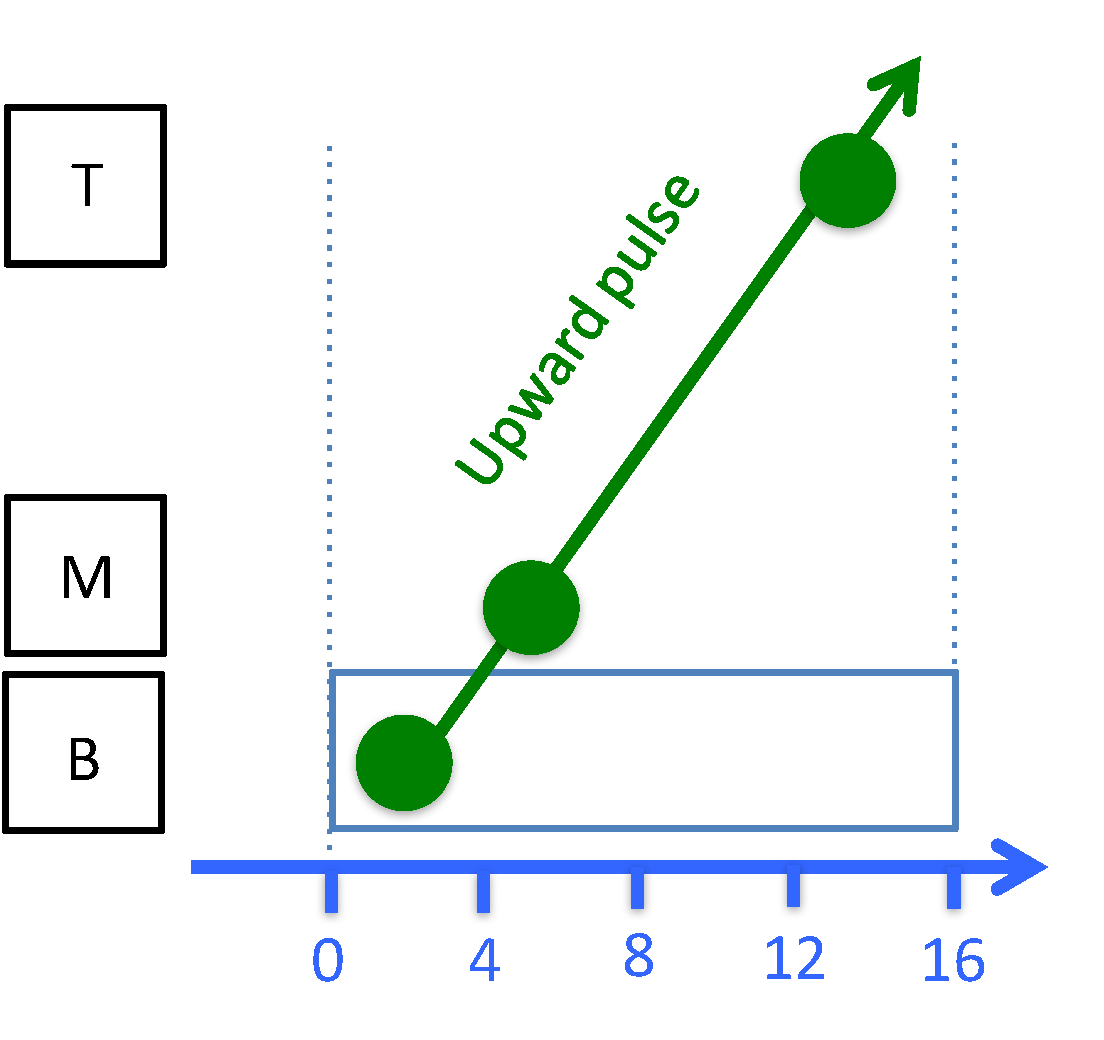
\includegraphics[width=.45\linewidth]{./Figs/ANITA3_l1trigger.pdf}
  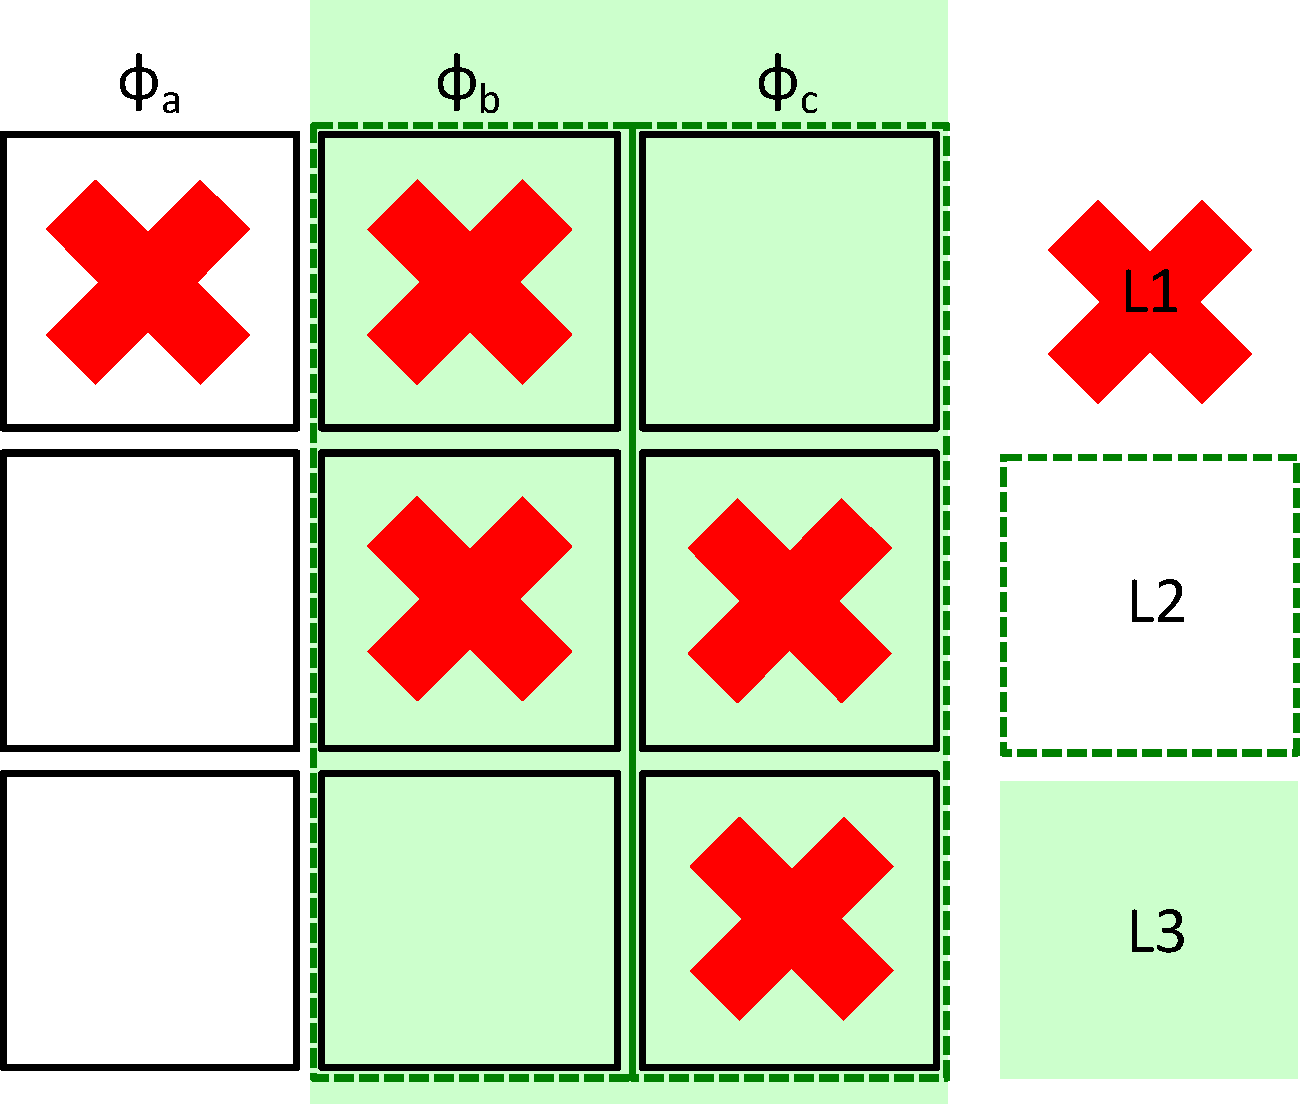
\includegraphics[width=.45\linewidth]{./Figs/ANITA3_globalTrigger.pdf}
  \caption{Schematic of a second-level trigger (left) example, where a
  plane-wave triggers an antenna in the bottom ring first, and a
  16\,ns window is opened to check L1 triggers in the middle and top
  ring.
The diagram on the right shows the issuance of a global trigger when two
adjacent azimuthal sectors had an L2 trigger.}
  \label{fig:ANITA_triggerLogic}
\end{figure}




%\subsubsection{Time dependent thresholds}
%\label{subsubsec:ANITA_thresholds}
%The ANITA-III flight softwares used an algorithm to vary the channel power thresholds during the flight and avoid overloading the DAQ in
%regions where the anthropogenic noise was higher.
%This algorithm tried to keep the scalers at roughly 500\,kHz.
%The current version of \icemc does not include anthropogenic noise or thermal variation coming from the Sun, but we still need to simulate the power threshold changes to have a more accurate simulation of our flights.

%In \icemc for every event, when picking the balloon position, the
%scalers for each channel are set by looking at sample data taken from the ANITA-III flight.
%The scalers are converted into relative power thresholds using
%a log function in the range 1-25\,MHz, assuming an exponential diode
%model with time constant $3.75 \times 10^{-9}$\,s.
%This was calculated from a fit to single channel power thresholds taken with
%an oscilloscope in 2008.

%Section~\ref{sec:validation} shows the variation of the acceptance when using the time-dependent thresholds or using constant thresholds throughout the simulated flight.

%Future versions of \icemc will include the simulation of anthropogenic noise, the contribution of the Sun, and a better treatment of the time varying thresholds.



